\chapter{Fluid Kinematics}
This chapter is based on Munson Chapter 4.

\section{The Velocity Field}

There are two ways of describing a fluid flow, the Eularian, and the Lagrangian approach:
\subsection{Difference Between Eularian and Lagrangian Approach}
For the Eularian approach, we define a velocity field which is a function of the three-dimensional position $\vec r$ and time $t$. From this we know where at which time the stream lines point in a certain direction.

The Lagrangian approach follows particles: A large amount of particles are released and traced as a function of time. 

\begin{figure}[H]
	\centering
	\begin{subfigure}{0.45\textwidth}
		\centering
		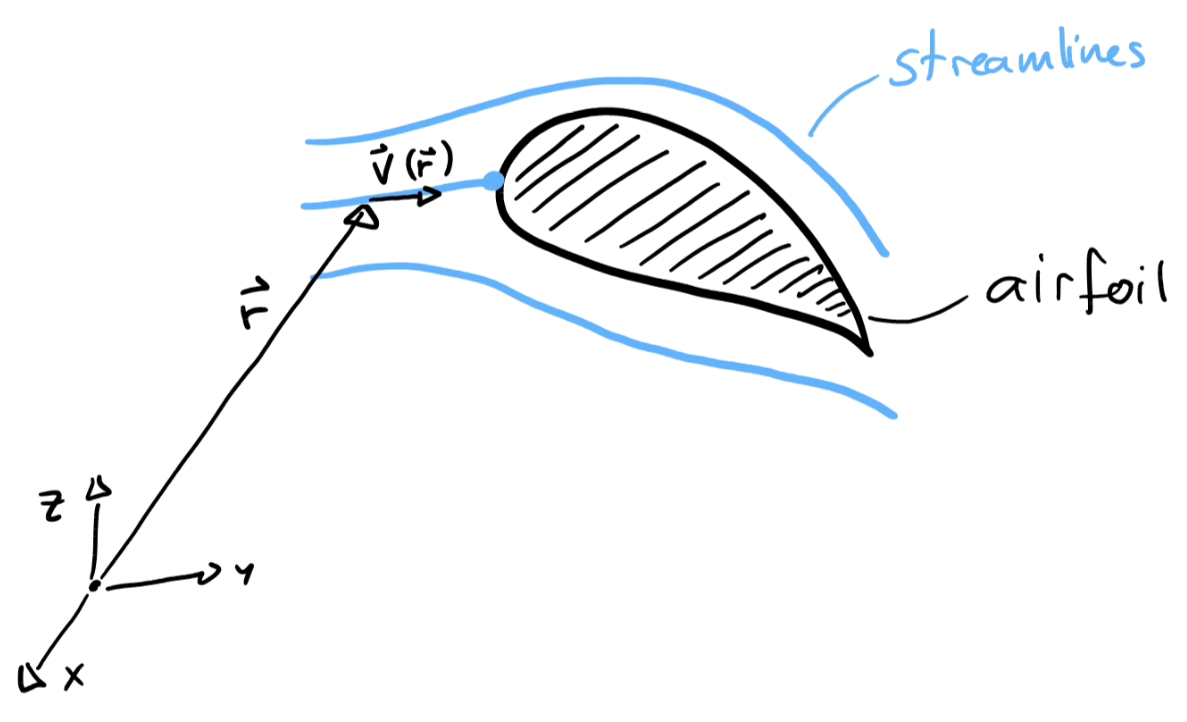
\includegraphics[width=\linewidth]{Sketches/EularianVelocityField}
		\begin{equation*}
			\vec V ( \vec r,t)
		\end{equation*}
		\caption{Eulerian velocity field}
		\label{fig:eularianvelocityfield}
	\end{subfigure}%
	\hfill
	\begin{subfigure}{0.45\textwidth}
		\centering
		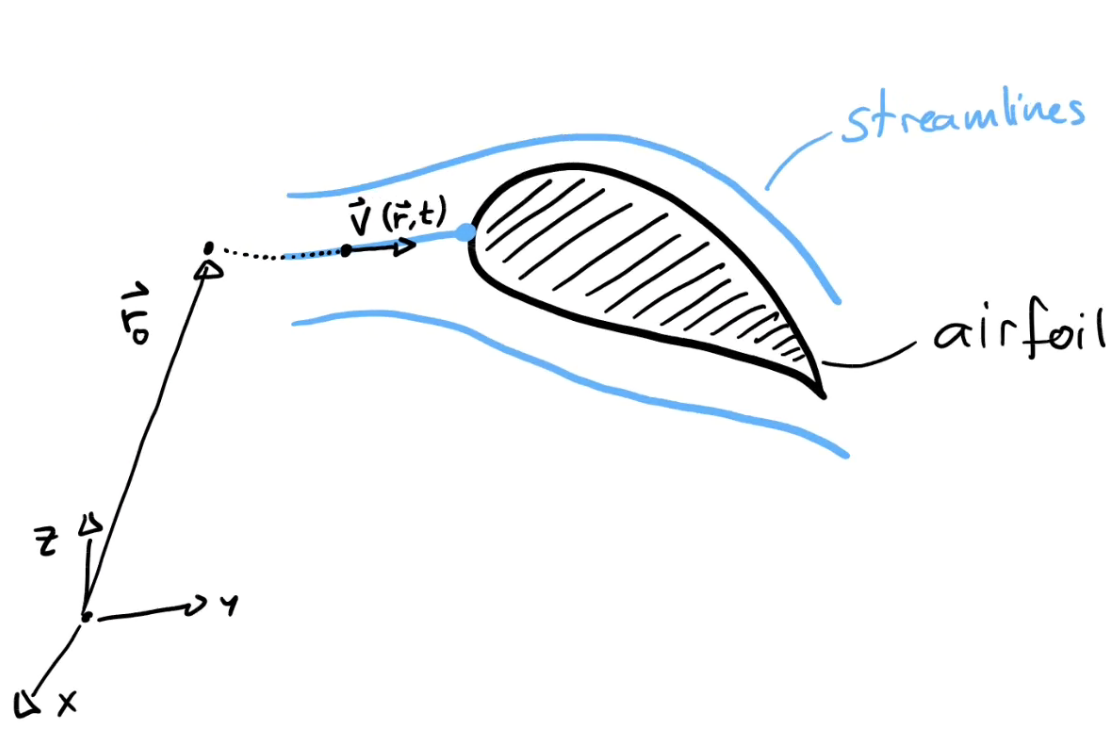
\includegraphics[width=\linewidth]{Sketches/LagrangianVelocityField}
		\begin{equation*}
			\vec V(\vec r_0,t)
		\end{equation*}
		\caption{Lagrangian velocity field}
		\label{fig:lagrangianvelocityfield}
	\end{subfigure}
	\caption{Comparison of (a) Eulerian and (b) Lagrangian velocity field representations}
	\label{fig:velocity_fields}
\end{figure}

\subsection{Visualizing Flows}
\begin{itemize}
	\item \textbf{Stream Line} (\textit{SL}) A line tangent to the velocity vector at any point.

	\begin{figure}[H]
			\centering
			\raisebox{-.5\height}{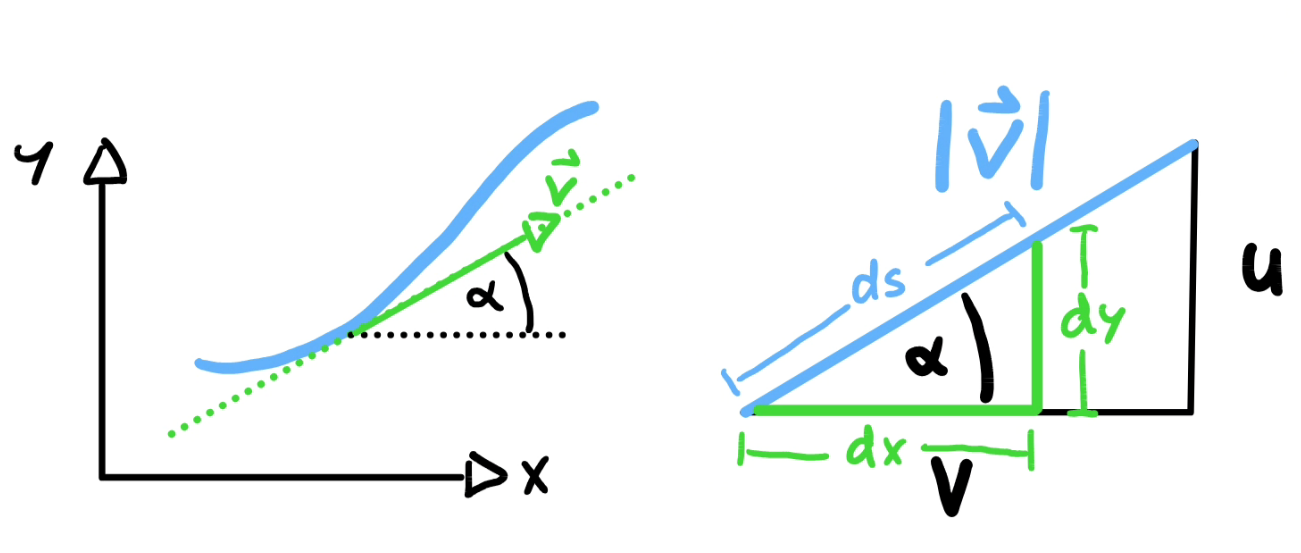
\includegraphics[width=0.45\linewidth]{Sketches/StreamLineEquationDerivation}}
			\label{fig:streamlineequationderivation}
	\end{figure}
	
	\begin{equation*}
		\frac{dy}{dx} = \frac vu\qquad \frac{dz}{dx} = \frac wu \qquad \frac{dz}{dy} = \frac wv
	\end{equation*}
	
	we can define the parametrised curve $\vec r_{sl}(s)$, described by:
	\begin{equation*}
		\frac{d\vec r_{sl}(s)}{ds} \times \vec V (\vec r_sp) = \vec 0
	\end{equation*}
	Stream lines are a purely Eurlarian concept.
	
	\item \textbf{Path Line} Line describing the actual path of a fluid element.

	\begin{equation*}
		\frac{d\vec r_p}{dt} = \vec V (\vec r_p(t))
	\end{equation*}
	where $V$ is the velocity at the instantaneous particle location and $\vec r_p$ is the position of a particle. In components this will result in:
	\begin{equation*}
		\frac{dx}{dt} = u\qquad \frac{dy}{dt} =v\qquad \frac{dz}{dt} = w
	\end{equation*}
	This is meant in a Lagrangian sense: We track a particle and register its position as a function of time.
	
	Similarly, we could write, as a ordinary differential equation:
	\begin{equation*}
		\frac{d\vec r_{pl}}{d t} = \vec V(\vec r_{pl},t)\qquad \text{where } \vec r_{pl} (t=t_0) = \vec r_{p_0}
	\end{equation*}
	
	
	\item \textbf{Steak Line} A line made up of particles, that have previously passed through a common point. It can be reconstructed from path lines: 
	\begin{equation*}
		\frac{d \vec \tau_p}{dt} = V(r_p,t)\qquad\text{width }\vec r_p(t=\tau_p) = \vec r_0\implies \vec r_p (t,\tau_p)
	\end{equation*}
\end{itemize}




\begin{figure}[H]
	\centering
	\begin{subfigure}{0.3\textwidth}	
		\centering
		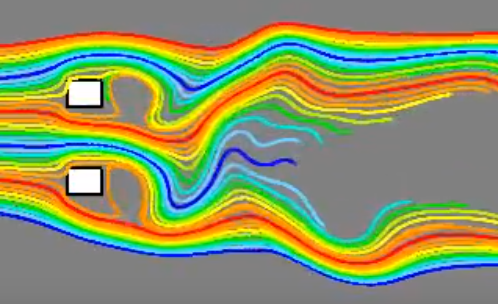
\includegraphics[width=\linewidth]{Sketches/StreamLine}
		\caption{Stream Line}
		\label{fig:streamlines}
	\end{subfigure}
	\hfill
	\begin{subfigure}{0.3\textwidth}
		\centering
		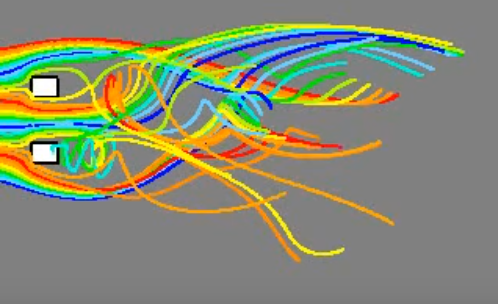
\includegraphics[width=\linewidth]{Sketches/PathLine}
		\caption{Path Line}
		\label{fig:pathline}
	\end{subfigure}%
	\hfill
	\begin{subfigure}{0.3\textwidth}
		\centering
		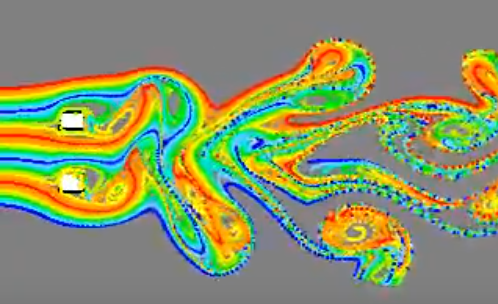
\includegraphics[width=\linewidth]{Sketches/StreakLine}
		\caption{Streak Line}
		\label{fig:streakline}
	\end{subfigure}
	\caption{Comparison of stream, path, and streak line.}
\end{figure}




